\documentclass[Second Project.tex]{subfiles}

\begin{document}

\subsection{ Πολυωνυμική Προσέγγιση }

Για την πολυωνυμική προσέγγιση χρησιμοποιείται η μέθοδος \textlatin{Newton}. Για $n$ σημεία 
εκπαίδευσης η μέθοδος αυτή παράγει ένα πολυώνυμο βαθμού $n-1$, το οποίο μάλιστα είναι και μοναδικό. 
Αρχικά υποθέτουμε ότι τα σημεία εκπαίδευσης προέρχονται από μία συνάρτηση $f(x)$, οπότε στόχος μας 
είναι να προσεγγίσουμε τα σημεία $(x_{1},f(x_{1})),\dots,(x_{n},f(x_{n}))$. Ορίζουμε ως 

\begin{equation*}
    f[x_{1} \hspace{5px}\dots\hspace{5px} x_{n}] 
\end{equation*}

τον συντελεστή του όρου $x^{n-1}$ στο πολυώνυμο που προσεγγίζει τα παραπάνω σημεία.

Ορίζοντας λοιπόν τα παραπάνω η μέθοδος \textlatin{Newton} ορίζει το ζητούμενο πολυώνυμο ως

\begin{equation*}
P(x) = f[x_{1}] + f[x_{1} \hspace{5px}x_{2}](x-x_{1}) + f[x_{1}\hspace{5px} \dots \hspace{5px} x_{n}](x-x_{1}) \dots (x-x_{n-1}) 
\end{equation*}

Όπου τα $f[x_{1}\hspace{5px} \dots \hspace{5px}x_{n}$] υπολογίζονται αναδρομικά ως εξής
\begin{equation*}
    f[x_{k} \hspace{5px} x_{k+1}] = \frac{f[x_{k+1}] - f[x_{k}]}{x_{k+1}-x_{k}}
\end{equation*}

Στο αρχείο \textlatin{\textbf{polynomial.py}} υπάρχουν τρεις συναρτήσεις. Η συνάρτηση \textlatin{\textit{polynomial\_interpolation}} δέχεται ως 
ορίσματα τα σημεία εκπαίδευσης και επιστρέφει τους συντελεστές του πολυωνύμου που προσεγγίζει αυτά τα σημεία. Οι συντελεστές του πολυωνύμου 
υπολογίζονται χρησιμοποιώντας το λεγόμενο τρίγωνο \textlatin{Newton}, το οποίο μοιάζει όπως το \textit{Σχήμα 1}. 

\vspace{5px}
\begin{figure}[h!]
    \centering
    \captionsetup{justification=centering}
    \begin{center}
        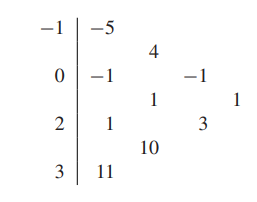
\includegraphics[scale=0.75]{newton_triangle.png}    
        \caption{ Τρίγωνο \textlatin{Newton} για 4 σημεία εκπαίδευσης ( Αριστερή στήλη η τιμή της ανεξάρτητης μεταβλητής των σημείων 
                                                                        εκπαίδευσης ) }
    \end{center}
\end{figure}

Από το οποίο παίρνουμε τα στοιχεία της πρώτης διαγωνίου ως συντελεστές του πολυωνύμου με τον σταθερό όρο του πολυωνύμου να είναι ο πρώτος 
όρος αυτής της διαγωνίου.Στην συνέχεια, η συνάρτηση \textlatin{\textit{calculate\_polynomial}} υπολογίζει και επιστρέφει την τιμή του 
πολυωνύμου στην τιμή $x$ που δέχεται ως παράμετρο χρησιμοποιώντας τον βαθμό του πολυωνύμου, τις τιμές της ανεξάρτητης μεταβλητής των σημείων 
εκπαίδευσης και τους συντελεστές του πολυωνύμου που υπολογίσθηκαν προηγουμένως. Τέλος, η συνάρτηση \textlatin{\textit{custom\_sin}} ορίζει 
αρχικά τα σημεία που αναφέρθηκαν στην παράγραφο της εισαγωγής της \textit{Άσκησης 1} και στην συνέχεια χρησιμοποιεί τις άλλες δύο συναρτήσεις 
για να προσεγγίσει την τιμή του ημιτόνου στο σημείο που δέχεται ως παράμετρο, αφού πρώτα το μεταφέρει στο διάστημα $[0,2\pi)$. 
\newpage
\end{document}